\hfill\break
\justifying
Como siguiente sección se colocan las funciones de filtrado. Los filtros son herramientas utilizadas para ayudar a eliminar o suavizar los efectos que tiene el ruido en una imagen.

\hfill\break
\justifying
Existen filtros que operan en el espectro frecuencial, otros en el espacial, etc. La clasificación que interesa en este trabajo será la de los filtros lineales y no lineales en el dominio espacial de los pixeles.

\hfill\break
\justifying
Los filtros en las imágenes pueden utilizarse para recorrer espectralmente la señal que interesa, consiguiéndose con la ayuda de un \textit{kernel}, que es simplemente una matriz pequeña que es convolucionada con la imagen para ejecutar un filtro adecuado.

\hfill\break
\justifying
Para los filtros que fueron implementados en el trabajo, se define siempre un \textit{kernel}, que se deja como un parámetro modificable por el usuario, pues la importancia que tiene el tamaño de este en el espectro de las frecuencias, equivaldría a modificar en un filtro analógico la frecuencia de corte.

\subsection*{Filtros lineales}
	
	\subsubsection*{Filtrado Promedio Aritmético}
		\hfill\break
		\justifying
		Considerado en la clasificación de filtros lineales, este tipo de filtro, ocupa un \textit{kernel} con valores unitarios en sus elementos, y se utiliza para la realización de la convolusión entre una ventana de la imagen y el \textit{kernel}.
		
		\hfill\break
		\justifying
		Esta convolusión resulta simplemente en la suma de todos los valores en esa ventana, aplicándoseles la división entre el número de elementos en la ventana y obteníendose el valor promedio que será asignado como nuevo valor al elemento ancla o central de la ventana.
		
		\begin{equation*}
			f_{pa} = \frac{1}{n^2} \sum_{(x,y)\in V} f(x,y)
		\end{equation*}
	
		La aplicación del filtro resulta visualmente en el desenfoque de la imagen, lo que se interpreta como el filtrado de las frecuencias más altas conservando aquellas más bajas.
		
	\subsubsection*{Filtro Gaussiano}
		\hfill\break
		\justifying
		El filtro gaussiano matemáticamente se define por la modificación de una señal de entrada por medio de una convolución con una función gausiana.
		
		\hfill\break
		\justifying
		Considerado el filtro ideal en el dominio del tiempo, tienen la propiedad de no sobrepasar la entrada de una función escalonada y al mismo tiempo disminuir el tiempo de subida y bajada.
		
		\hfill\break
		\justifying
		En el procesamiento de imágenes, cada elemento de la matriz representa un atributo de píxel, como el brillo o la intensidad del color, y el efecto generl que se obtiene de su implementación se le denomina desenfoque gaussiano.
		
		
	\begin{landscape}
		\hfill\break
		\hfill\break
		\hfill\break
		\begin{figure}[!h]
			\begin{tabular}{cc}
				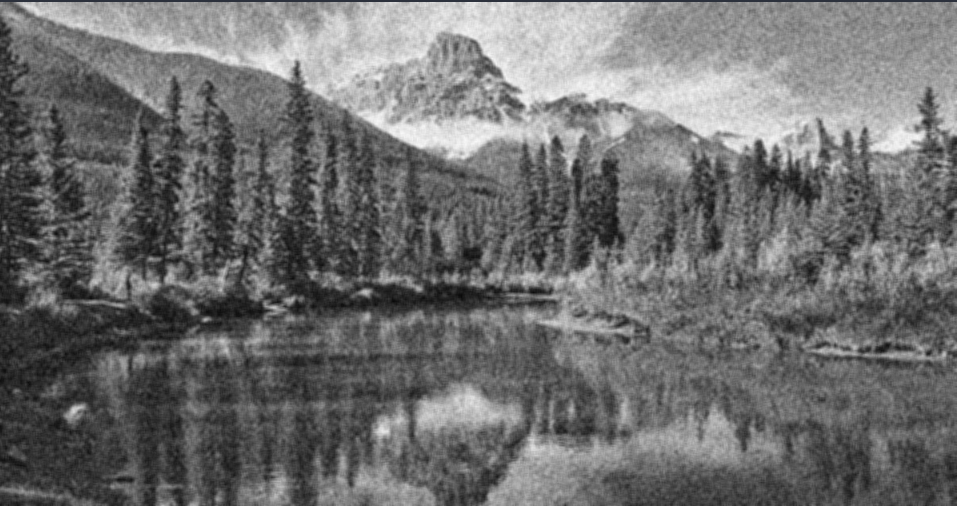
\includegraphics[width=12.25cm]{Imagenes/Ruido_Gauss_5_50_FMA_5.png} & 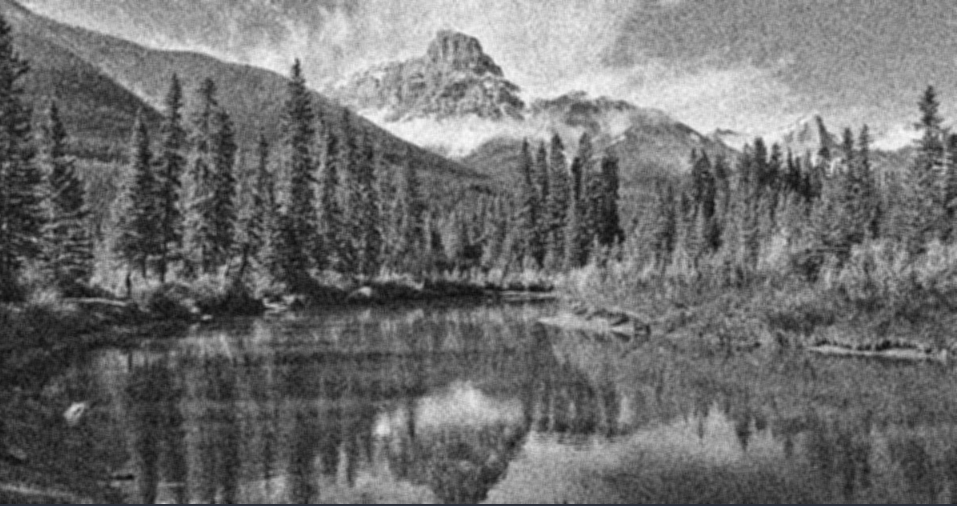
\includegraphics[width=12.25cm]{Imagenes/Ruido_Gauss_5_50_Gauss_5_5.png} \\
				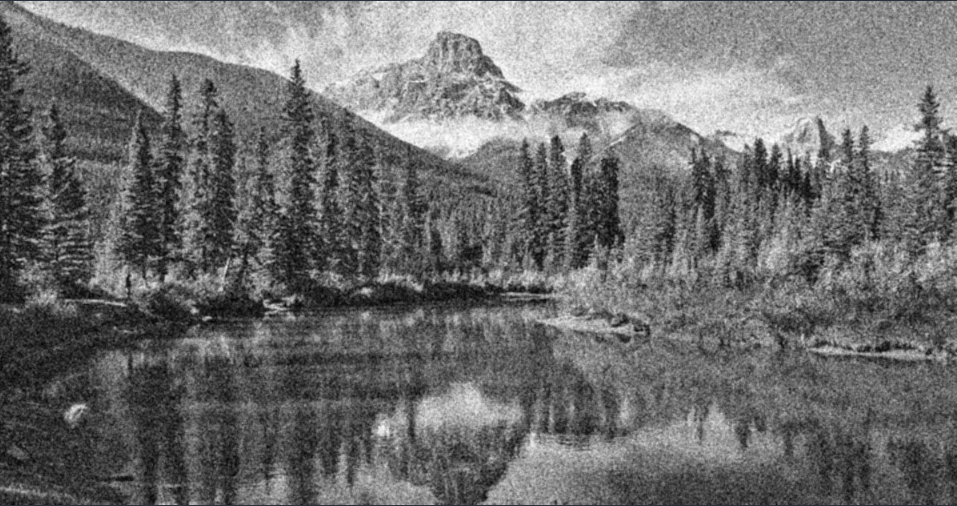
\includegraphics[width=12.25cm]{Imagenes/Ruido_Gauss_5_50_FMA_3.png} & 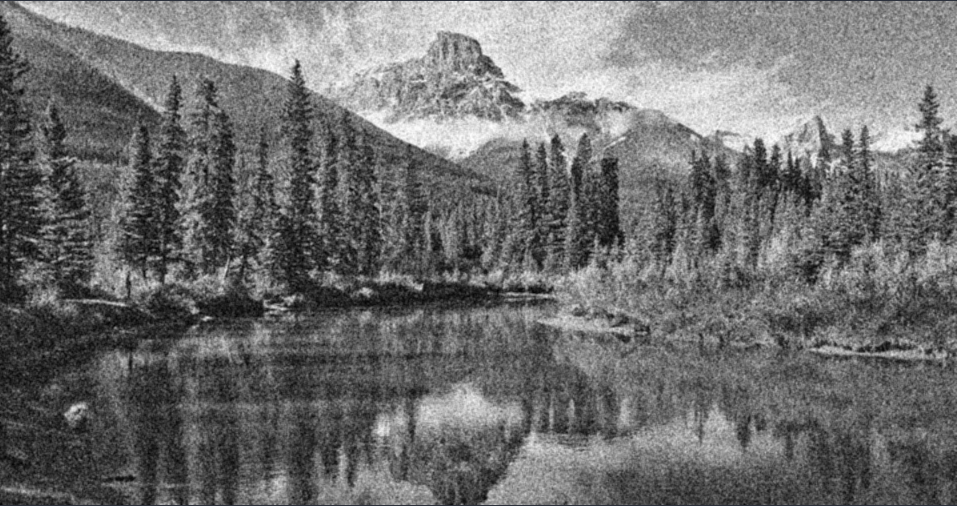
\includegraphics[width=12.25cm]{Imagenes/Ruido_Gauss_5_50_Gauss_5_3.png}
			\end{tabular}
			\label{Ruido_Gauss_Filtros_lineales}
			\caption{Ejemplo de imágenes adicionadas con ruido Gaussiano con $\mu = 5$ y $\sigma = 50$ y los filtros lineales. \\ 1) Imagen filtrada con el Filtro Media Aritmética y tamaño de \textit{kernel} $n = 5$ \\ 2) Imagen filtrada utilizando el Filtro Gaussiano con parámetros $\sigma = 5$ y tamaño de \textit{kernel} $n = 5$ \\ 3) Imagen filtrada con el Filtro Media Aritmética y tamaño de \textit{kernel} $n = 3$ \\ 4)Imagen filtrada utilizando el Filtro Gaussiano con parámetros $\sigma = 5$ y tamaño de \textit{kernel} $n = 3$}
		\end{figure}
		
		\newpage
		
		\begin{figure}[!h]
			\begin{tabular}{cc}
				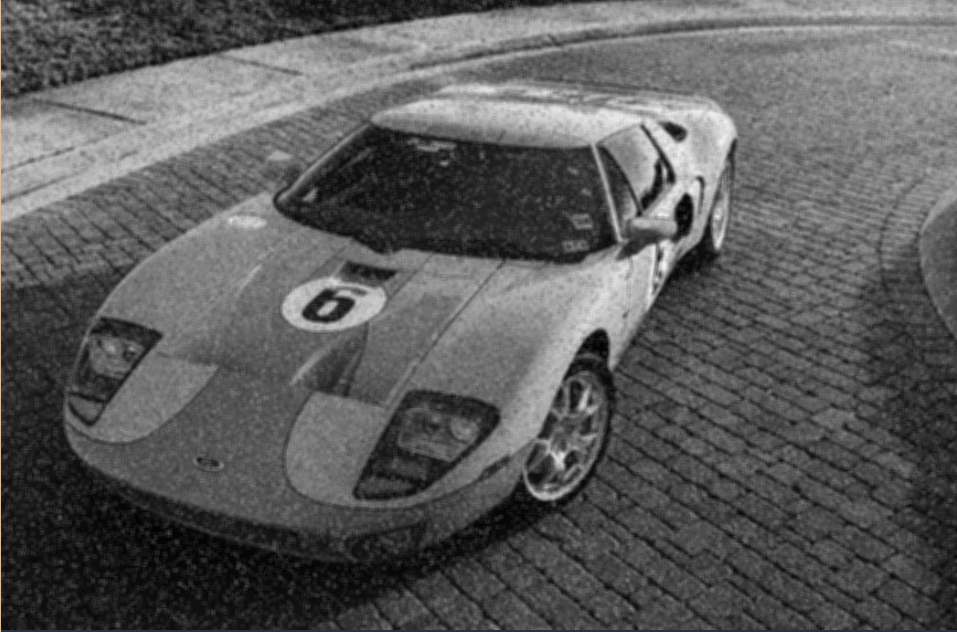
\includegraphics[width=12.25cm]{Imagenes/Ruido_sp_25_FMA_5.png} & 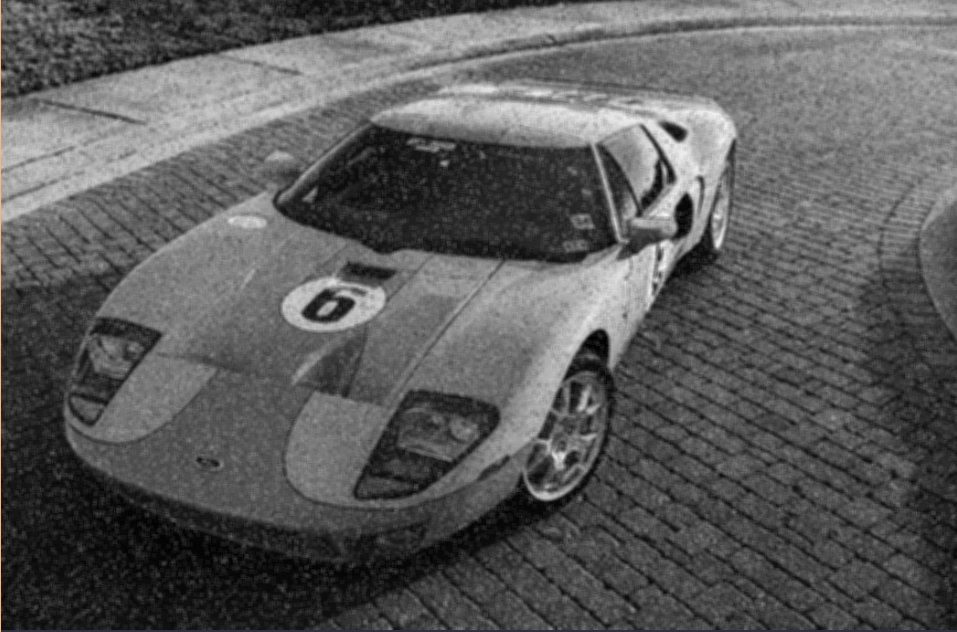
\includegraphics[width=12.25cm]{Imagenes/Ruido_sp_25_Gauss_5_5.png} \\
				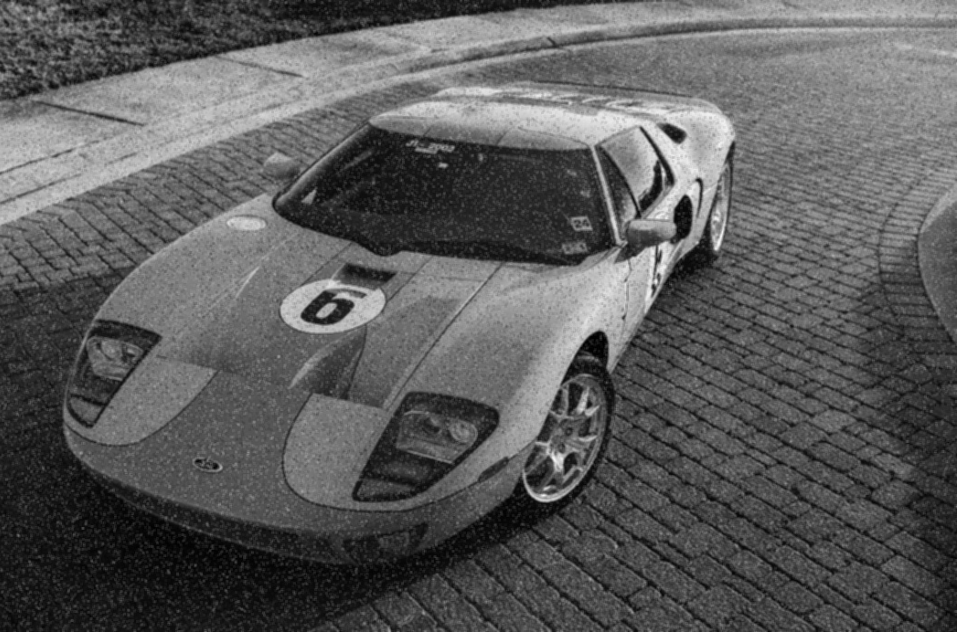
\includegraphics[width=12.25cm]{Imagenes/Ruido_sp_25_FMA_3.png} & 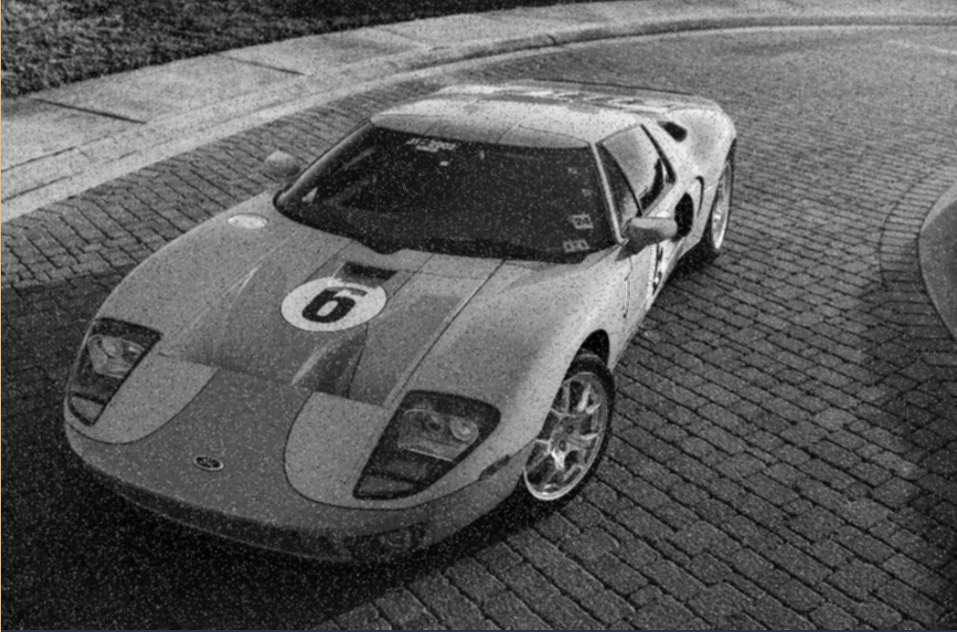
\includegraphics[width=12.25cm]{Imagenes/Ruido_sp_25_Gauss_5_3.png}
			\end{tabular}
			\label{Ruido_SalPimienta_Filtros_lineales}
			\caption{Ejemplo de imágenes adicionadas con ruido Sal y Pimienta, con $l = 25$ y los filtros lineales. \\ 1) Imagen filtrada con el Filtro Media Aritmética y tamaño de \textit{kernel} $n = 5$ \\ 2) Imagen filtrada utilizando el Filtro Gaussiano con parámetros $\sigma = 5$ y tamaño de \textit{kernel} $n = 5$ \\ 3) Imagen filtrada con el Filtro Media Aritmética y tamaño de \textit{kernel} $n = 3$ \\ 4)Imagen filtrada utilizando el Filtro Gaussiano con parámetros $\sigma = 5$ y tamaño de \textit{kernel} $n = 3$}
		\end{figure}
	\end{landscape}

	\subsection*{Filtros no lineales}
		\hfill\break
		\justifying
		Un filtro no lineal es aquel cuya salida no es una función lineal de su entrada. Este tipo de filtros suelen tener muchas aplicaciones especialmente en ruidos no aditivos.
		
		\hfill\break
		\justifying
		En comparación con los filtros lineales, estos tienen un comportamiento muy distinto, siendo la características más importante para estos, la salida del filtro o la respuesta del filtro no obedece a principios como la escala y la invarianza. Este tipo de filtros pueden producir resultados que varian de una manera no intuitiva.
		
		\hfill\break
		\justifying
		El principio general de operación de los filtros no lineales de orden es:
		\begin{enumerate}
			\item Ordenamiento de los valores dentro de la ventana de valore desordenados
			\item Elegir una regla para la selección de algún valor
			\item Asignación del el nuevo valor en la imagen de salida
		\end{enumerate}
	
		\subsubsection*{Filtro Mediana}
			\hfill\break
			\justifying
			Este filtro tiene un comportamiento muy sencillo, que equivale a ordenar los valores dentro de la ventana en forma ascedente, y tomar como nuevo valor del elemento central el elemento mediano de la secuencia.
			
			\hfill\break
			\justifying
			Suelen obtener buenos resultados para imágenes con ruido Sal y Pimienta.
			
		\subsubsection{Filtros Max y Min}
			\hfill\break
			\justifying
			Iniciando con el mismo proceso, se ordena la secuencia en forma ascendente y se toman los valores extremos en cada filtro. Para el filtro Max, se toma el último valor, el más grande, mientras que para el filtro Min el primero.
		
		\begin{figure}[!h]
			\begin{tabular}{cc}
				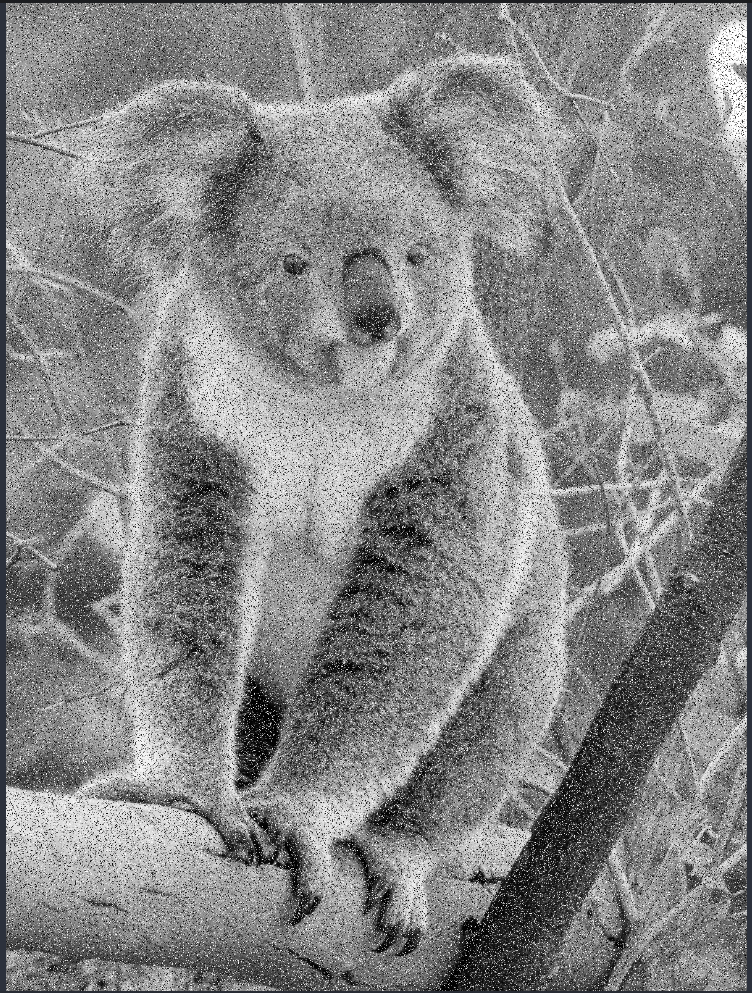
\includegraphics[width=8.5cm]{Imagenes/Ruido_sp_10_.png} & 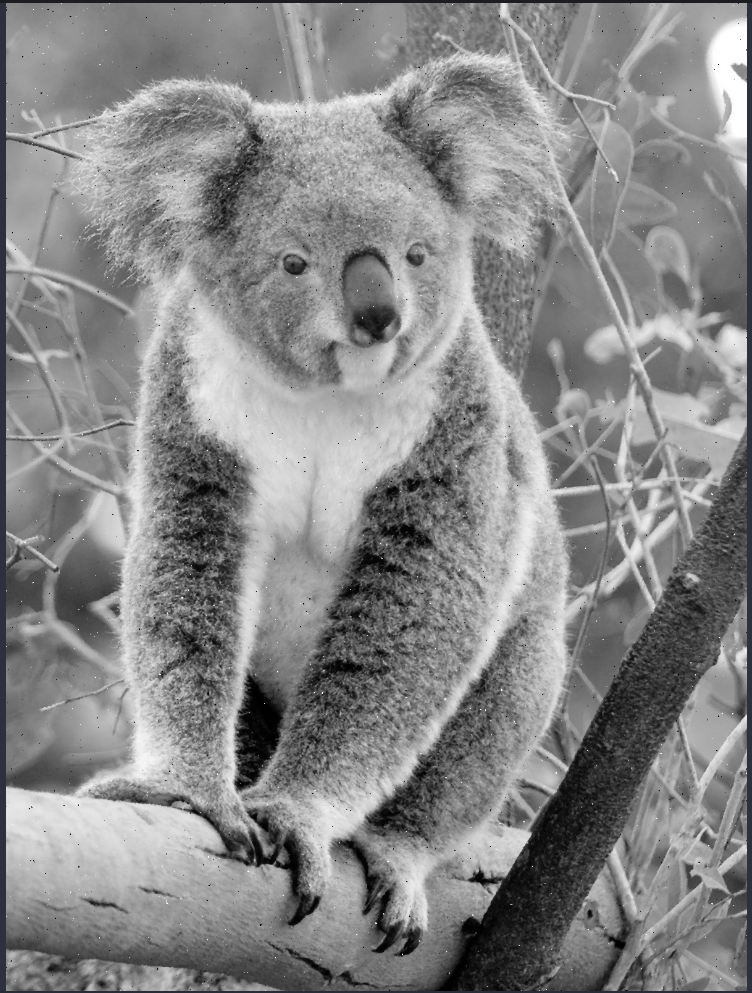
\includegraphics[width=8.5cm]{Imagenes/Ruido_sp_10_mediana_3.png} \\
			\end{tabular}
			\label{Ruido_SP_Filtro_no_lineale_mediana}
			\caption{Ejemplo de una imágene adicionada con una gran cantidad de ruido Sal y Pimienta con $l = 10$ y más sin embargo con el uso del filtro mediano con \textit{kernel} tamaño $n=3$ se logra eliminar una gran cantidad de ruido}
		\end{figure}
		
	\begin{landscape}
		\hfill\break
		\hfill\break
		\hfill\break
		\hfill\break
		\begin{figure}[!h]
			\centering
			\begin{tabular}{ccc}
				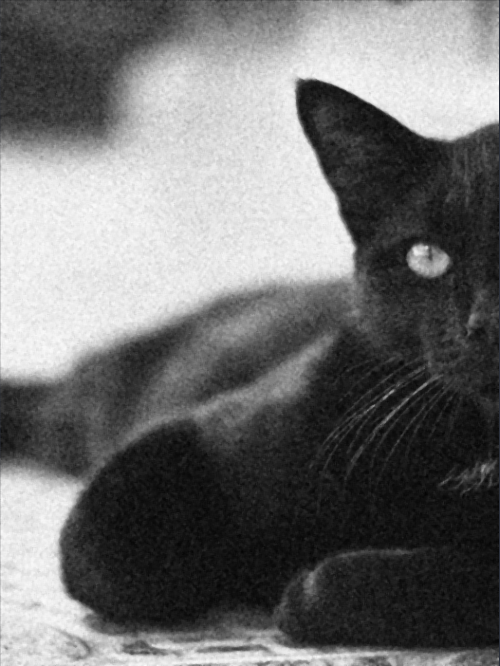
\includegraphics[width=8cm]{Imagenes/Ruido_Gauss_5_50_mediana_5.png} & 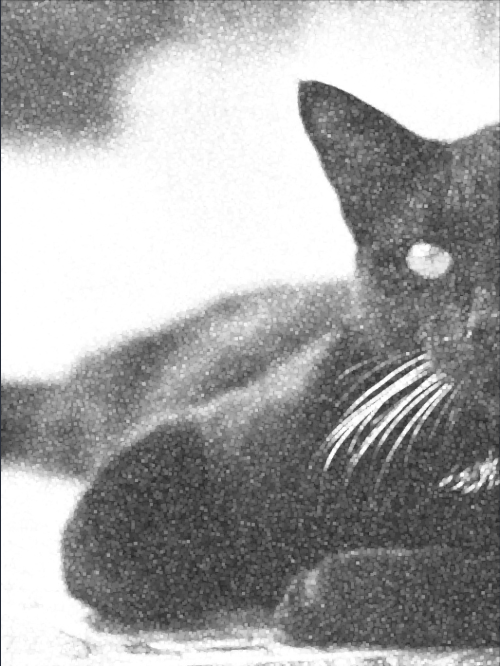
\includegraphics[width=8cm]{Imagenes/Ruido_Gauss_5_50_max_5.png} &
				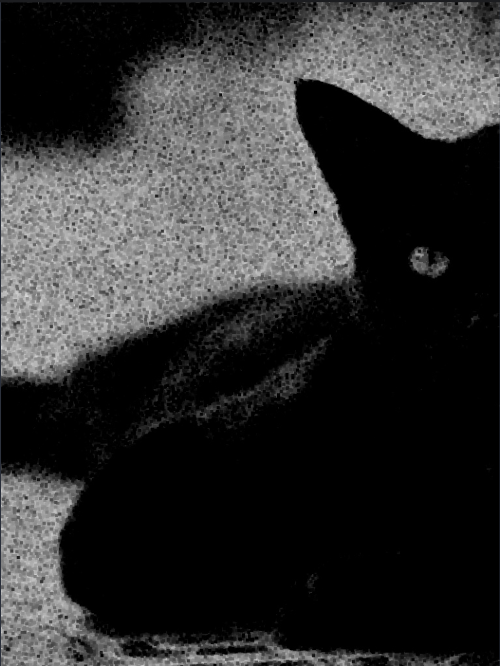
\includegraphics[width=8cm]{Imagenes/Ruido_Gauss_5_50_min_5.png}
			\end{tabular}
			\label{Ruido_Gauss_Filtros_no_lineales}
			\caption{Ejemplo de imágenes adicionadas con ruido Gaussiano con $\mu = 5$ y $\sigma = 50$ y los filtros no lineales de orden. \\ 1) Imagen filtrada con el Filtro Mediana con tamaño de \textit{kernel} $n = 5$ \\ 2) Imagen filtrada utilizando el Filtro Max con tamaño de \textit{kernel} $n = 5$ \\ 3) Imagen filtrada con el Filtro Min con tamaño de \textit{kernel} $n = 5$ }
		\end{figure}
	
		\newpage
		
		\begin{figure}[!h]
			\begin{tabular}{cc}
				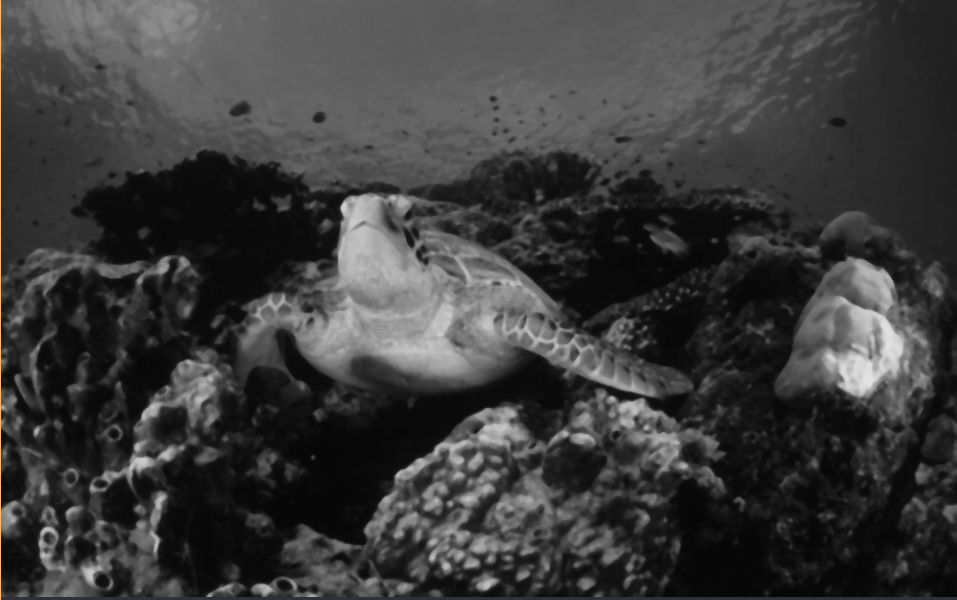
\includegraphics[width=12.25cm]{Imagenes/Ruido_sp_50_mediana_5.png} & 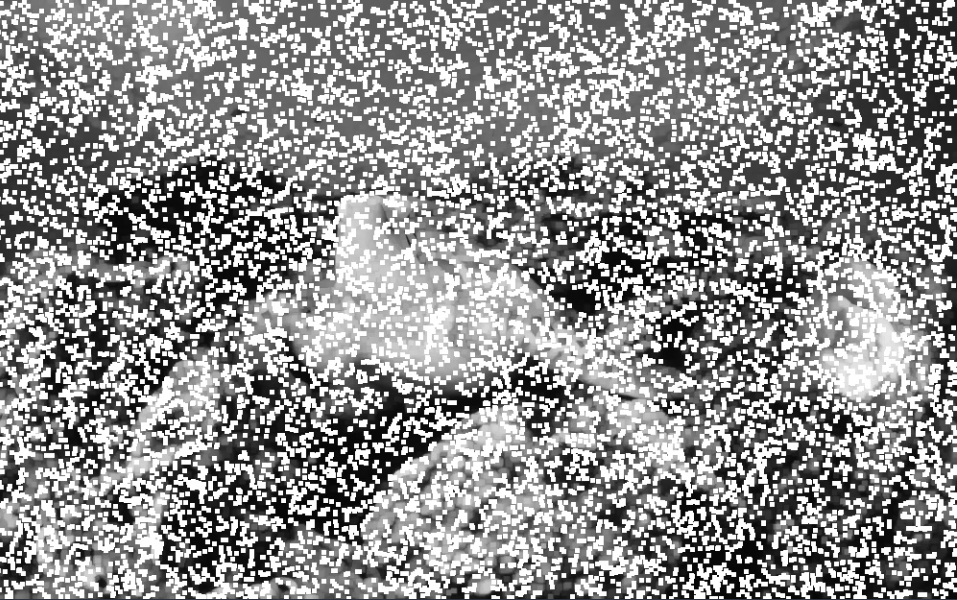
\includegraphics[width=12.25cm]{Imagenes/Ruido_sp_50_max_5.png} \\
				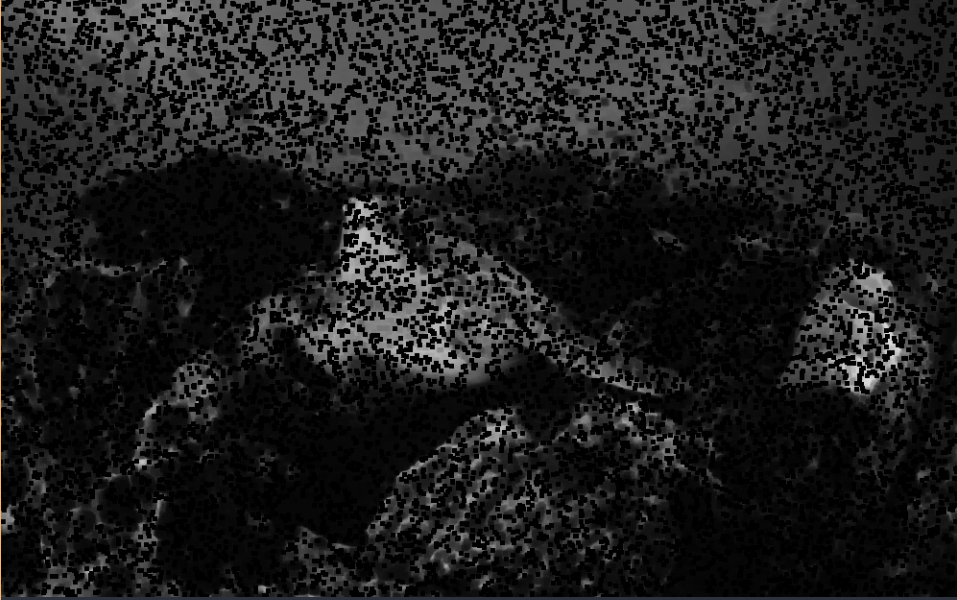
\includegraphics[width=12.25cm]{Imagenes/Ruido_sp_50_min_5.png} & 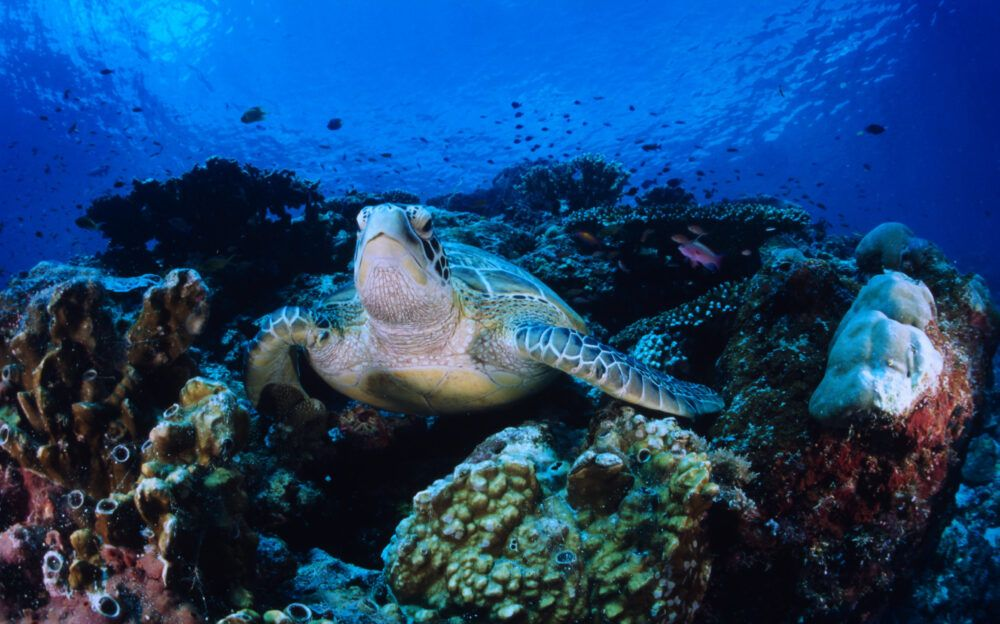
\includegraphics[width=12.25cm]{Imagenes/tortuga.jpeg}
			\end{tabular}
			\label{Ruido_SalPimienta_Filtros_no_lineales}
			\caption{Ejemplo de imágenes adicionadas con ruido Sal y Pimienta, con $l = 50$ y los filtros no lineales de orden. \\ 1) Imagen filtrada con el Filtro Mediana con tamaño de \textit{kernel} $n = 5$ \\ 2) Imagen filtrada utilizando el Filtro Max con tamaño de \textit{kernel} $n = 5$ \\ 3) Imagen filtrada con el Filtro Min con tamaño de \textit{kernel} $n = 5$ \\ 4) Fotografía original de tortuga nadando entre arrecifes. }
		\end{figure}
	\end{landscape}

	\begin{lstlisting}[language=Python]
		def filtering(filter_type:str,image,n:int=3,**kargs):
			image = copy(image)
			
			if filter_type == 'mean':
				# Kernel creation
				#   Before applying any convolution with an image using a 2D matrix it's needed to ensure 
				#   all the values are normalize, thus the division of the matrix
				kernel = ones((n,n),float32)/(n**2)
				# Mean filtering
				#   ddepth: a -1 value means the final image will also have the same depth as the original
				return cv2.filter2D(image,-1,kernel)
			elif filter_type == 'gaussian':
				std_deviation = 0 if 'std_deviation' not in list(kargs) else kargs['std_deviation']
				return cv2.GaussianBlur(image,(n,n),std_deviation)
			elif filter_type == 'median':
				return cv2.medianBlur(image,n)
			elif filter_type == 'max':
				# The morphological dilation is equivalent to a maximum filter
				kernel = cv2.getStructuringElement(cv2.MORPH_RECT,(n,n))
				return cv2.dilate(image,kernel)
			elif filter_type == 'min':
				# The morphological erosion is equivalent to a minimum filter
				kernel = cv2.getStructuringElement(cv2.MORPH_RECT,(n,n))
				return cv2.erode(image,kernel)
	\end{lstlisting}